\chapter{Developed work}
\label{chapter:developed_work}

\section{How to add formatted code}

In the developed work section you will probably want to add some code you developed. You can use the listings package to do this. 

\begin{lstlisting}[language=Python]
import numpy as np
	
def incmatrix(genl1,genl2):
	m = len(genl1)
	n = len(genl2)
	M = None #to become the incidence matrix
	VT = np.zeros((n*m,1), int)  #dummy variable
	
	#compute the bitwise xor matrix
	M1 = bitxormatrix(genl1)
	M2 = np.triu(bitxormatrix(genl2),1) 

	for i in range(m-1):
		for j in range(i+1, m):
			[r,c] = np.where(M2 == M1[i,j])
			for k in range(len(r)):
				VT[(i)*n + r[k]] = 1;
				VT[(i)*n + c[k]] = 1;
				VT[(j)*n + r[k]] = 1;
				VT[(j)*n + c[k]] = 1;
				
				if M is None:
					M = np.copy(VT)
				else:
					M = np.concatenate((M, VT), 1)
				
				VT = np.zeros((n*m,1), int)
	
	return M
\end{lstlisting}

This example was taken from the Overleaf documentation, \href{https://www.overleaf.com/learn/latex/Code_listing}{here}.

\section{How to add a directory trees}

Check this project's directory tree in Figure \ref{fig:directory_structure} for more information on each file.

\begin{figure}[!htb]
    \dirtree{%
    .1 /.
	.2 .vscode\DTcomment{VSCode settings. Delete it if you're not using VSCode}.
	.3 \dots.
    .2 images\DTcomment{Store your images here}.
	.3 \dots.
	.2 .gitignore\DTcomment{Some files shouldn't be saved to the repo. Here is a template .gitignore file}.
	.2 .latexmkrc\DTcomment{RC file for latexmk. If you're using Overleaf you don't need this.}.
    .2 abstract.tex.
	.2 acronyms.tex\DTcomment{Acronym entries go here}.
	.2 appendices.tex.
	.2 conclusion.tex.
	.2 cover.tex\DTcomment{Document cover page}.
	.2 developed\_work.tex.
	.2 glossary.tex\DTcomment{Glossary entries go here}.
	.2 introduction.tex.
	.2 literature\_review.tex.
	.2 Makefile\DTcomment{Project's makefile needed to compile project to pdf}.
	.2 nomenclature.tex\DTcomment{Nomenclature entries go here}.
	.2 preamble.tex\DTcomment{File with all needed packages and custom commands}.
	.2 references.bib\DTcomment{Bibliography file}.
	.2 results.tex.
	.2 resumo.tex\DTcomment{Abstract in Portuguese}.
	.2 thesis.pdf\DTcomment{Output pdf file}.
	.2 thesis.synctex.gz\DTcomment{Synctex file needed to navigate directly from code to pdf and vice-versa}.
	.2 thesis.tex\DTcomment{Project's main file which calls all other files}.
    }

    \caption{This project's directory structure.}
    \label{fig:directory_structure}
\end{figure}

\section{How to add tables}

You can create a table using \LaTeX. Use \href{https://www.tablesgenerator.com/}{this} \LaTeX table generator to help you out.

\begin{table}[!htb]
	\centering
	\caption{A simple table with dummy values.}
	\begin{tabular}{|l|l|l|}
		\hline
			  & column 1 & column 2 \\ \hline
		row 1 & 1        & 2        \\ \hline
		row 2 & 3        & 4        \\ \hline
	\end{tabular}
	\label{tab:simple_table}
\end{table}

You can also include tables which are images instead of tabulars. To do this, create your own table, screenshot it and include it in your document as a table (as opposed to a figure). Like this:

\begin{table}[!htb]
	\centering
	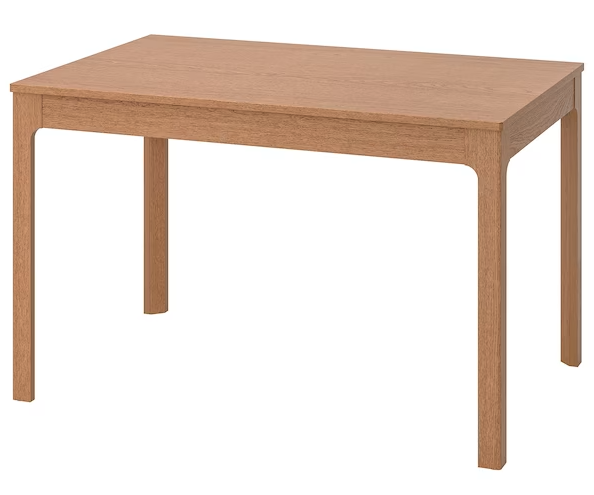
\includegraphics[width=0.5\textwidth]{images/table.png}
	\caption{Another simple table. As you can see anything can be a table in \LaTeX! Don't lose too much time trying to create all your tables using the tabular environment.}
	\label{tab:table_table}
\end{table}

\begin{tcolorbox}[title=A note on table captions]
	Most people prefer table captions to show above the table itself. However, since the guide provided by Técnico (which you can find \href{https://tecnico.ulisboa.pt/en/education/study-at-tecnico/academic-information/masters-dissertation/}{here}) doesn't specify a specific placement, this is a matter of opinion. If you want your table caption to be above the table use the example of Table \ref{tab:simple_table}, otherwise use the example of Table \ref{tab:table_table}.
\end{tcolorbox}
